\documentclass[float=false, crop=true]{standalone}

\usepackage{tikz}
\usetikzlibrary{positioning, shapes.geometric}

\begin{document}
\begin{figure}
    \centering
    \scriptsize
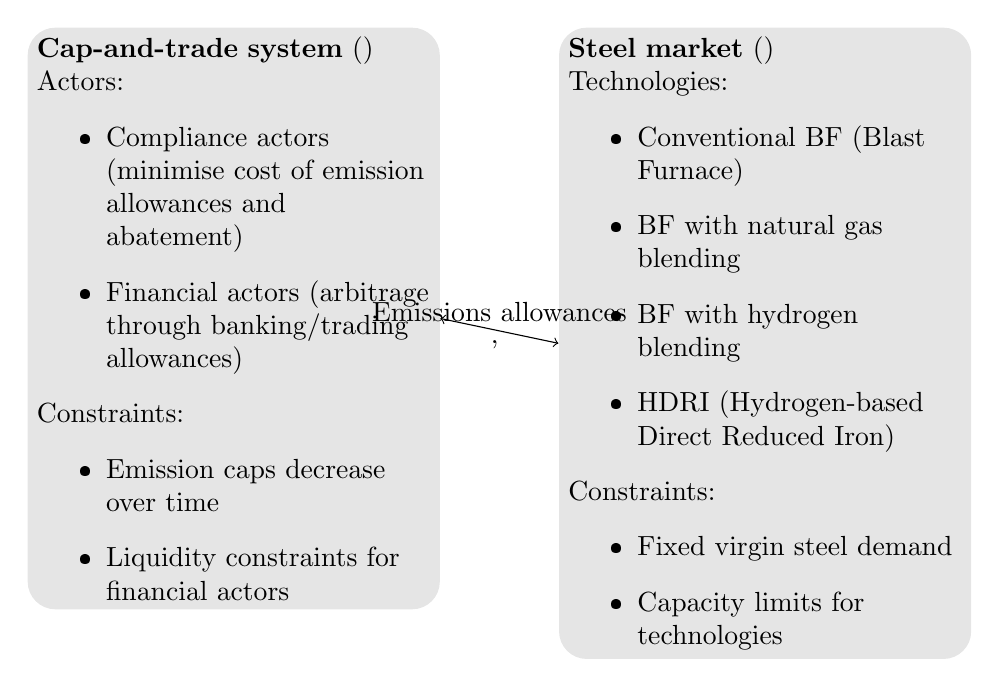
\begin{tikzpicture}[
square/.style={rectangle, rounded corners=10, fill=gray!20, text=black, minimum height=1.5cm, text width=5cm,align=left},
mainsquare/.style={rectangle, rounded corners=10, fill=gray!20, text=black, minimum height=3cm, text width=5cm,align=left},
subsquare/.style={rectangle, rounded corners=10, draw=black, dashed, text=black, minimum height=1.5cm, text width=5cm,align=left}
]

% Cap-and-trade system
\node[mainsquare] (ets) [below] {\textbf{Cap-and-trade system $(\pets)$}\\
Actors:
\begin{itemize}
    \item Compliance actors (minimise cost of emission allowances and abatement)
    \item Financial actors (arbitrage through banking/trading allowances)
\end{itemize}
Constraints:
\begin{itemize}
    \item Emission caps decrease over time
    \item Liquidity constraints for financial actors
\end{itemize}
};

% Steel market
\node[mainsquare, fill=gray!20] (steel) [right=1.5cm of ets.north east, anchor=north west] {\textbf{Steel market $(\psteel)$}\\
Technologies:
\begin{itemize}
    \item Conventional BF (Blast Furnace)
    \item BF with natural gas blending
    \item BF with hydrogen blending
    \item HDRI (Hydrogen-based Direct Reduced Iron)
\end{itemize}
Constraints:
\begin{itemize}
    \item Fixed virgin steel demand
    \item Capacity limits for technologies
\end{itemize}
};

% Connections
\draw[<->] (ets.east) -- (steel.west) node[midway, above] {Emissions allowances} node[midway, below] {$\bis$, $\bfs$};

\end{tikzpicture}
\end{figure}
\end{document}